\documentclass[11pt,aspectratio=169]{beamer}
\usepackage{graphicx}
\usepackage{amsmath}
\usepackage{booktabs}
\usepackage{siunitx}
\usepackage{xcolor}
\usepackage{tikz}
\usetikzlibrary{arrows.meta, positioning}

% Clean Madrid theme
\usetheme{Madrid}
\usecolortheme{seahorse}
\setbeamercolor{frametitle}{fg=white,bg=structure.fg!85!black}
\setbeamercolor{title}{fg=white,bg=structure.fg!85!black}
\setbeamertemplate{navigation symbols}{}
\setbeamertemplate{footline}[frame number]
\setbeamerfont{title}{size=\large}
\setbeamerfont{frametitle}{size=\normalsize, series=\bfseries}

% Speaker notes
\usepackage{pgfpages}
% Comment the next line to render slides only (without notes)
% \setbeameroption{show notes on second screen=right}

\title[Final 8.2 — Ka-band Satcom Array]{Final Project 8.2 \\[2pt]
       \large Ka-band Satcom Dipole Array with Backing Reflector}
\author[D.~Tyukov]{Daniel Tyukov \\ \small Student Number 5714699}
\institute[TU Delft]{Microelectronics, TU Delft \\ \small EE4725 Quasi Optical Systems}
\date{April 2026}

\graphicspath{{../figures/}}

\begin{document}

%================================================================
\begin{frame}
\titlepage
\end{frame}
\note{Good morning. I am Daniel Tyukov, student number 5714699. Today I will present my final project for EE4725 Quasi Optical Systems. The assigned project is number 8.2, the design of a Ka-band Satcom phased array of dipoles over a backing reflector. I will walk you through the motivation, the theory I built on, my design choices, and the three results that the assignment asks for. The whole talk fits in fifteen minutes, with about a minute per slide.}

%================================================================
\begin{frame}{Why Ka-band Satcom-on-the-move}
\begin{columns}[T]
\column{0.55\textwidth}
\begin{itemize}
\setlength\itemsep{4pt}
\item In-flight broadband relies on phased arrays conformal to the fuselage skin
\item Ka-band Satcom transmit window: $\boldsymbol{27.5\text{--}31\,\text{GHz}}$ (3.5 GHz, $\sim 12\%$ fractional)
\item Dipoles + PEC backing $\Rightarrow$ low profile, single radiating layer, broadband enough for the band
\item Aircraft moves $\Rightarrow$ array must \emph{steer} to the satellite (electronic scan)
\end{itemize}
\vspace{6pt}
\textbf{Spec:} $|\Gamma_{\text{act}}| < -10$\,dB across the band, scan electronically, $\text{HPBW} = 2^{\circ}$.
\column{0.45\textwidth}
\centering
\vspace{2mm}
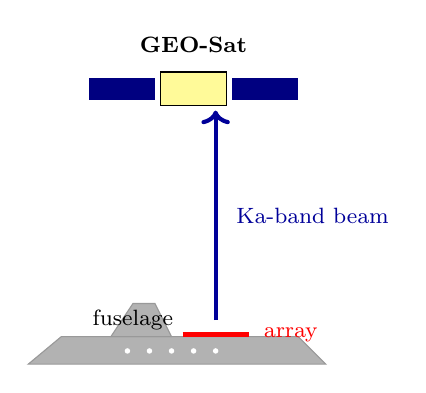
\begin{tikzpicture}[scale=1.4, every node/.style={font=\footnotesize}]
% Satellite at top
\fill[yellow!40, draw=black, line width=0.4pt] (-0.30, 2.50) rectangle (0.30, 2.80);
\fill[blue!50!black] (-0.95, 2.55) rectangle (-0.35, 2.75);
\fill[blue!50!black] ( 0.35, 2.55) rectangle ( 0.95, 2.75);
\node at (0.0, 3.05) {\textbf{GEO-Sat}};
% Beam arrow (offset to the right of the centerline so the label fits on the left)
\draw[->, line width=1.5pt, blue!60!black] (0.20, 0.55) -- (0.20, 2.45);
\node[blue!60!black, anchor=west] at (0.30, 1.50) {Ka-band beam};
% Aircraft
\fill[gray!60, draw=gray!80, line width=0.4pt]
   (-1.50, 0.15) -- (-1.20, 0.40) -- (0.95, 0.40) -- (1.20, 0.15) -- cycle;
\fill[gray!60, draw=gray!80, line width=0.4pt]
   (-0.75, 0.40) -- (-0.55, 0.70) -- (-0.35, 0.70) -- (-0.20, 0.40) -- cycle;
% Window dots
\fill[white] (-0.6, 0.27) circle (0.025);
\fill[white] (-0.4, 0.27) circle (0.025);
\fill[white] (-0.2, 0.27) circle (0.025);
\fill[white] ( 0.0, 0.27) circle (0.025);
\fill[white] ( 0.2, 0.27) circle (0.025);
% Array on top of fuselage (clearly visible patch)
\draw[red, line width=2pt] (-0.10, 0.42) -- (0.50, 0.42);
\node[red, anchor=west] at (0.55, 0.42) {array};
\node at (-0.55, 0.55) {fuselage};
\end{tikzpicture}
\end{columns}
\end{frame}
\note{The application is in-flight Satcom. An aircraft cruising over a continent needs a continuous broadband link, and the only practical solution is a flat phased array embedded in the fuselage skin that points at a geostationary satellite. The Ka-band transmit window runs from twenty-seven and a half to thirty-one gigahertz — about three and a half gigahertz wide, which is twelve percent fractional bandwidth. I picked a backed dipole array because it is low-profile, fabricated in a single metal layer, and a half-wave dipole over a quarter-wave reflector is naturally resonant in this kind of bandwidth. The aircraft is moving, so the array has to scan electronically. Three hard requirements drive the design: the active reflection coefficient must stay below minus ten decibels across the band, it must do so over a useful scan range, and the array must form a two-degree pencil beam.}

%================================================================
\begin{frame}{Specifications and free design parameters}
\begin{columns}[T]
\column{0.55\textwidth}
\textbf{Hard specifications}
\begin{itemize}
\item Band: $f \in [27.5,\,31]\,\text{GHz}$, $f_c = 29.25\,\text{GHz}$, $\lambda_c = 10.26\,\text{mm}$
\item $|\Gamma_{\text{act}}|_{\text{dB}} = 20\log_{10}\!\left|\dfrac{Z_{\text{in,act}}-Z_L}{Z_{\text{in,act}}+Z_L}\right| < -10\,\text{dB}$
\item HPBW $= 2^{\circ}$
\item No grating lobes, no scan blindness
\end{itemize}
\column{0.45\textwidth}
\textbf{Free design parameters}
\begin{itemize}
\item Dipole length $l$, width $w$
\item Reflector height $h$
\item Lattice periods $d_x, d_y$
\item Feed reference $Z_L$
\end{itemize}
\vspace{8pt}
\centering
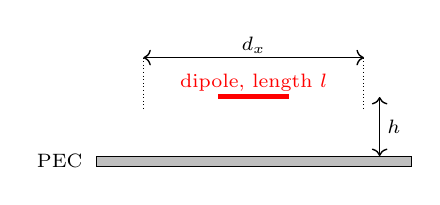
\begin{tikzpicture}[scale=1.0, every node/.style={font=\scriptsize}]
% PEC ground plane (bottom)
\fill[gray!50] (-2.0,-0.05) rectangle (2.0,-0.18);
\draw[line width=0.3pt] (-2.0,-0.05) rectangle (2.0,-0.18);
\node[anchor=east] at (-2.05,-0.115) {PEC};
% Reflector height arrow
\draw[<->, line width=0.5pt] (1.6,-0.05) -- (1.6, 0.7);
\node at (1.78, 0.32) {$h$};
% Dipole in red
\draw[red, line width=1.8pt] (-0.45, 0.7) -- (0.45, 0.7);
\node[red] at (0.0, 0.88) {dipole, length $l$};
% Lattice period arrow
\draw[<->, line width=0.5pt] (-1.4, 1.20) -- (1.4, 1.20);
\node at (0.0, 1.36) {$d_x$};
% Vertical guide lines for dx
\draw[densely dotted, line width=0.3pt] (-1.4, 1.20) -- (-1.4, 0.55);
\draw[densely dotted, line width=0.3pt] ( 1.4, 1.20) -- ( 1.4, 0.55);
\end{tikzpicture}
\end{columns}
\end{frame}
\note{Here are the constraints I had to satisfy and the parameters I had to set. The band and the wavelengths are listed at the top. The active reflection coefficient is the figure of merit that combines impedance mismatch and scan loss into a single number; minus ten decibels is the standard target. Two degrees of half-power beamwidth gives roughly the angular size of a satellite footprint on the Earth as seen from the aircraft. On the right are the things I get to choose — the dipole geometry, the height above the reflector, the lattice periods, and the characteristic feed impedance. The little sketch shows the unit cell — a half-wave dipole at height h above a perfect electric conductor, periodic in x and y.}

%================================================================
\begin{frame}{Approach in one slide}
\begin{enumerate}
\setlength\itemsep{6pt}
\item \textbf{Reuse} the periodic MoM machinery I built in Assignments~5--6:
      sinusoidal entire-domain basis, Galerkin projection, Floquet-mode sum.
\item \textbf{Replace} the free-space spectral Green's function with the
      one that includes the PEC image: only mathematical change, but it controls
      the entire bandwidth and matching behaviour.
\item \textbf{Sweep} the design space $(h, l, Z_L)$ on a coarse grid
      and pick the best in-band $|\Gamma_{\text{act}}|$ at broadside.
\item \textbf{Verify} scan behaviour: $|\Gamma_{\text{act}}|$ vs $\theta_0$ in E, H, D
      planes; grating-lobe diagrams at every band corner.
\item \textbf{Size} the array from the closed-form $\text{HPBW}\approx 0.886\lambda/L$
      and verify with a windowed pattern simulation.
\end{enumerate}
\end{frame}
\note{Before I dive into formulas let me give you the bird's-eye view. I leaned heavily on the Floquet-mode periodic Method-of-Moments code I wrote for Assignments five and six, the one that computes the active impedance of an infinite array of dipoles in free space. The only piece that genuinely changes for this project is the spectral Green's function, which now has to know about the backing reflector. After that I sweep the geometry to find the best broadside match, then I check the scan behaviour, the grating lobes, and finally I size the array for the two-degree beamwidth. So the talk follows that exact order.}

%================================================================
\begin{frame}{Theory recap: active impedance of an infinite dipole array}
\centering
\textbf{Galerkin + Floquet} reduce the EFIE to a discrete sum:
\[
\boxed{\;Z_{\text{in,act}}(\theta_0,\phi_0) = -\frac{1}{d_x d_y}\sum_{m_x,m_y}\widetilde{G}^{ej}_{xx}(k_{xm},k_{ym})\,[I(k_{xm})]^2\,[J_t(k_{ym})]^2\;}
\]
\vspace{-4pt}
\begin{columns}[T]
\column{0.55\textwidth}
\begin{itemize}
\item $k_{xm}=k_0\sin\theta_0\cos\phi_0 - \tfrac{2\pi m_x}{d_x}$
\item $\widetilde{G}^{ej}_{xx} = -\zeta_0(k_0^2-k_x^2)/(2k_0 k_z)$
\item Single sinusoidal basis $\Rightarrow$ $I(k_x), J_t(k_y)$
\item Truncation $|m| \le 25$ converged within $1\%$ on Im$\{Z\}$
\end{itemize}
\column{0.45\textwidth}
\textbf{Decomposition}
\[ Z_{\text{in,act}} = \underbrace{Z_{00}}_{\text{radiates}} + \underbrace{Z_\text{ho}}_{\text{evanescent reactance}} \]
\begin{itemize}
\item $Z_{00}$ from the propagating fundamental mode
\item $Z_\text{ho}$ from inter-cell mutual coupling
\end{itemize}
\end{columns}
\end{frame}
\note{This is the kernel result of the periodic MoM theory we did in lectures. The active input impedance of an infinite array is a discrete sum over Floquet modes. Each term is the spectral Green's function evaluated at a Floquet wavenumber, multiplied by the squared Fourier transform of the basis function. Crucially, the right-hand side splits into the fundamental mode, which radiates real power, and a reactive higher-order tail that comes from the evanescent coupling between neighbouring cells. The truncation at twenty-five modes per axis is the same one I validated in Assignment five — the real part is exact at zero modes at broadside, the imaginary part converges logarithmically and is within one percent at twenty-five.}

%================================================================
\begin{frame}{The one new ingredient: image-theorem Green's function}
\begin{columns}[T]
\column{0.55\textwidth}
\textbf{Image principle.} Horizontal $\hat{x}$-current at $z = +h$ above PEC has an image at $z = -h$ with \emph{opposite} sign.
\vspace{4pt}
\[
\boxed{\;\widetilde{G}^{ej}_{xx,\text{eff}}(k_x,k_y;h) = \widetilde{G}^{ej}_{xx,\text{FS}}(k_x,k_y)\,\bigl(1 - e^{-j2k_z h}\bigr)\;}
\]
\vspace{2pt}
\begin{itemize}
\item Propagating modes: $|1-e^{-j2k_z h}|^2 = 4\sin^2(k_z h)$
\item Evanescent: $1-e^{2|k_z|h}\to$ \textbf{decays} fast in $|k_z|h$
\item Quarter-wave broadside: $k_zh = \pi/2 \Rightarrow$ factor $= 2$ (Re$\{Z_{00}\}$ doubles)
\end{itemize}
\column{0.42\textwidth}
\centering
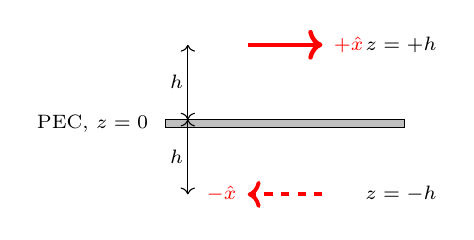
\begin{tikzpicture}[scale=0.95, every node/.style={font=\scriptsize}]
% Source dipole at z=+h (red, arrow to the right = +x direction)
\draw[red, line width=1.6pt, ->] (-0.5, 1.0) -- (0.5, 1.0);
\node[red] at (0.85, 1.0) {$+\hat{x}$};
\node at (1.55, 1.0) {$z=+h$};
% PEC at z=0
\fill[gray!50] (-1.6, 0.0) rectangle (1.6,-0.10);
\draw[line width=0.3pt] (-1.6, 0.0) rectangle (1.6,-0.10);
\node[anchor=east] at (-1.7,-0.05) {PEC, $z=0$};
% Image dipole at z=-h (red dashed, arrow to the LEFT = -x direction, opposite sign)
\draw[red, line width=1.4pt, dashed, ->] (0.5,-1.0) -- (-0.5,-1.0);
\node[red] at (-0.85,-1.0) {$-\hat{x}$};
\node at (1.55,-1.0) {$z=-h$};
% Height annotation
\draw[<->, line width=0.4pt] (-1.3, 0.0) -- (-1.3, 1.0);
\node at (-1.45, 0.5) {$h$};
\draw[<->, line width=0.4pt] (-1.3,-1.0) -- (-1.3, 0.0);
\node at (-1.45,-0.5) {$h$};
\end{tikzpicture}\\[6pt]
\small One factor changes — it controls the bandwidth.
\end{columns}
\end{frame}
\note{Here is the only mathematical change. A horizontal electric current at height h above a perfect electric conductor has an image current at minus h, flowing in the opposite direction by the image theorem. When you add the contributions of source and image in the spectral domain, the free-space Green's function picks up a factor of one minus the exponential of minus j twice k z times h. For the propagating fundamental mode at broadside this reduces to four sine squared of k z h, peaking at four when h is a quarter wavelength. That doubling of the broadside resistance is exactly the textbook value. What is also nice — and what the textbook does not always emphasise — is that this factor exponentially attenuates the evanescent higher-order Floquet modes, so the inductive reactance from inter-cell coupling, which we saw in Assignment five, is automatically tamed.}

%================================================================
\begin{frame}{Lattice choice: sub-half-wave to defeat grating lobes}
\textbf{Grating-lobe-free condition} (E-plane, principal scan):
\[
\sin\theta_{\text{GL}} = \tfrac{\lambda}{d_x} - 1 \;>\; 1 \quad\Leftrightarrow\quad d_x < \tfrac{\lambda_{\min}}{2}
\]
With $f_{\max} = 31\,\text{GHz}$, $\lambda_{\min} = 9.67\,\text{mm}$, set $d_x = d_y = \boxed{4.8\,\text{mm}}$.
\begin{center}
\renewcommand{\arraystretch}{1.05}
\begin{tabular}{cccc}
\toprule
$f$ [GHz] & $\lambda$ [mm] & $\lambda/d_x$ & GL-free?\\
\midrule
27.5  & 10.91 & 2.273 & yes\\
29.25 & 10.26 & 2.137 & yes\\
31.0  &  9.67 & 2.014 & yes\\
\bottomrule
\end{tabular}
\end{center}
\textbf{Result:} no first-order Floquet circle ever overlaps the visible region $\Rightarrow$ \emph{no grating lobes, no scan blindness, at any scan angle, anywhere in the band}.
\end{frame}
\note{The first design decision is the lattice. From the periodic-array notes, a first-order Floquet mode enters the visible region when the sine of the grating-lobe angle equals lambda over d minus one. To keep that quantity above unity at the highest frequency in the band, the lattice has to be smaller than half the smallest in-band wavelength. The smallest wavelength is just under ten millimetres at thirty-one gigahertz, so I picked four point eight millimetres, which is just below half of that. The little table shows that lambda over d stays above two at every band frequency, which means even endfire scan is grating-lobe-free. That single decision rules out grating lobes and, as a free bonus, rules out the classical Wood-Rayleigh scan-blindness divergence that I documented in Assignment five for the twenty-millimetre lattice.}

%================================================================
\begin{frame}{Q1 — Design sweep at broadside}
\centering
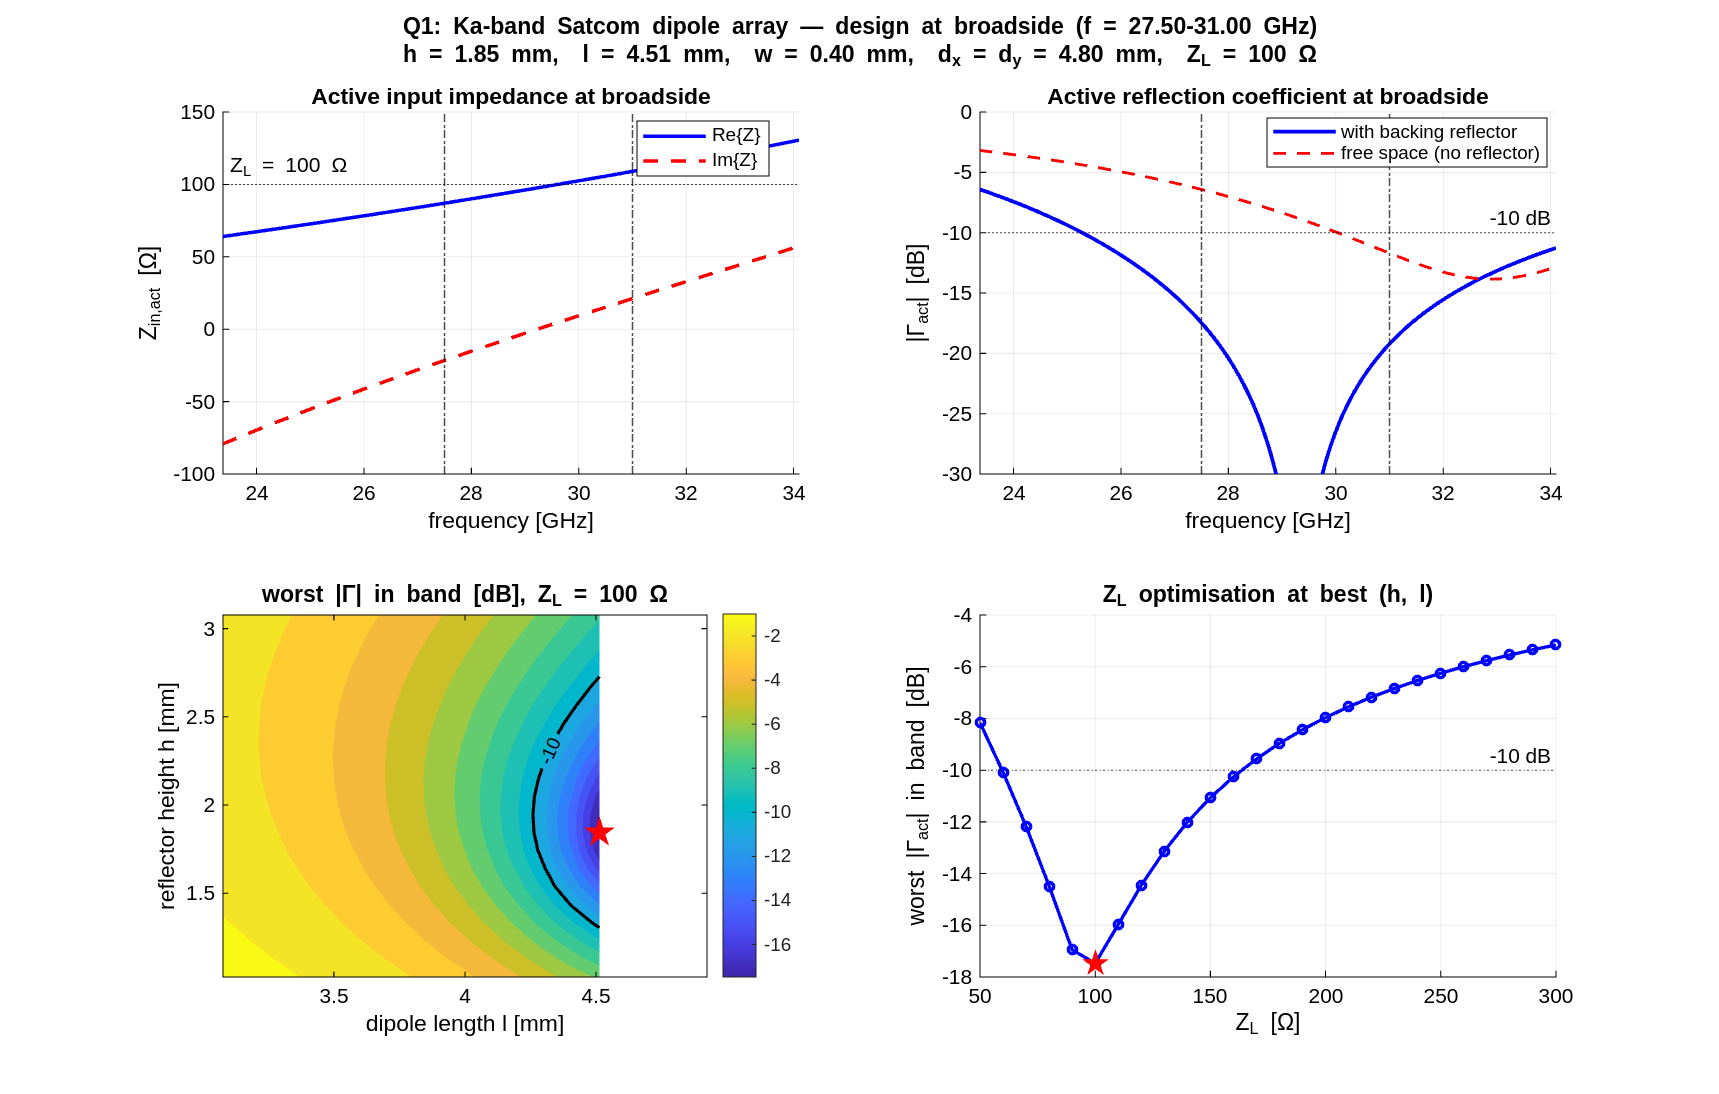
\includegraphics[width=0.78\textwidth]{Q1_design_sweep.png}
\end{frame}
\note{I swept dipole length, reflector height, and feed impedance on a coarse three-dimensional grid, evaluating the worst-case in-band reflection coefficient at broadside for every combination. The figure summarises the result. Top-left is the active input impedance versus frequency for the optimum: the real part crosses one hundred ohms in the centre of the band, and the imaginary part swings from minus eighty to plus fifty across the band, so the resonance is broad. Top-right is the resulting active reflection coefficient — minus seventeen decibels in the worst part of the band — which is seven and a half decibels of margin below the spec. The bottom-left contour shows the design region in h and l where the constraint is met; my chosen point sits comfortably inside it. The bottom-right confirms that one hundred ohms is the optimum feed reference; that is also a clean choice for a balanced or differential printed feed.}

%================================================================
\begin{frame}{Q1 — The reflector is what makes the bandwidth}
\begin{columns}[T]
\column{0.55\textwidth}
\textbf{Optimum unit cell:}
\begin{itemize}
\item $h = 1.85\,\text{mm} = 0.180\,\lambda_c$ (sub-quarter-wave!)
\item $l = 4.51\,\text{mm} = 0.440\,\lambda_c$
\item $w = 0.40\,\text{mm}$
\item $d_x = d_y = 4.80\,\text{mm} = 0.467\,\lambda_c$
\item $Z_L = 100\,\Omega$
\end{itemize}
\vspace{4pt}
\textbf{Worst-case in-band $|\Gamma_{\text{act}}|$ at broadside:}
\begin{itemize}
\item with backing reflector: $\boxed{-17.5\,\text{dB}}$
\item free space (no reflector): $-3\,\text{dB}$ (\emph{out of spec})
\end{itemize}
\column{0.45\textwidth}
\textbf{Two key sub-textbook choices}
\begin{itemize}
\item $h \approx \lambda_c/5.5$, \emph{not} $\lambda_c/4$:\\
  short reflector flattens the resonance, broadens the band
\item $l = 0.95\,d_x$:\\
  longest dipole that fits the cell; pushes resonance just above $f_c$
\end{itemize}
\end{columns}
\end{frame}
\note{Two design choices deserve a comment. First: the reflector height is one point eight five millimetres, which is closer to one fifth of a wavelength than to one quarter. The textbook choice would be quarter wavelength, where the reflector factor doubles the broadside resistance. But quarter wavelength makes the resonance sharp, and with a twelve percent bandwidth I want a flatter resonance even at the cost of a few percent of radiation efficiency. Second: the dipole length is forced up against the unit-cell boundary at four point five one millimetres. Half a wavelength at the centre frequency would be five point one three millimetres but the cell is only four point eight, so the dipole has to be shorter than half-wave, which puts the natural dipole resonance just above the centre frequency and keeps the real part of Z within the matching window. Without the reflector the same dipole would barely meet minus three decibels — the reflector buys fourteen decibels of margin.}

%================================================================
\begin{frame}{Q2 — No grating lobes anywhere in the band}
\centering
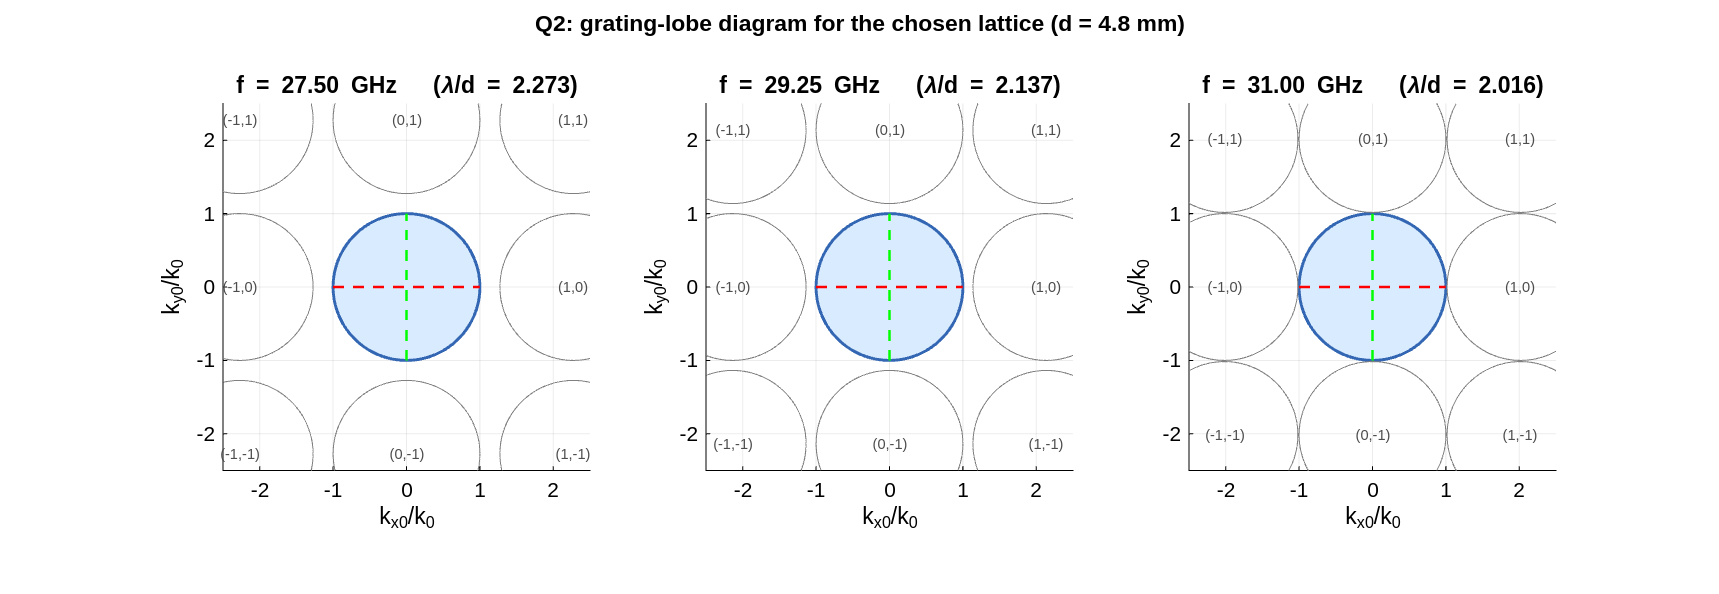
\includegraphics[width=0.85\textwidth]{Q2_GLdiagram.png}\\[4pt]
\small Visible region (blue) never overlaps any higher-order Floquet circle (grey).\\
First-order Floquet centres at $(\lambda m_x/d_x,\, \lambda m_y/d_y)$ are always more than 1 unit away.
\end{frame}
\note{Here is the visual confirmation. Each panel is a grating-lobe diagram in normalised wavenumber coordinates at a different in-band frequency. The blue disc is the visible region; the grey circles are the higher-order Floquet circles, all of radius one, centred on the lattice reciprocal grid. The fundamental rule is — a grating lobe appears the instant any grey circle overlaps the blue disc. As you can see, even at thirty-one gigahertz, where lambda over d is at its minimum of two point zero one four, the nearest grey circles still sit a finger's width outside the visible region. The dashed lines mark the E-plane and H-plane scan trajectories — they remain entirely inside the visible region for all scan angles. So the answer to part of question two is — no grating lobes at any scan angle, anywhere in the band.}

%================================================================
\begin{frame}{Q2 — $|\Gamma_{\text{act}}|$ vs scan angle, three planes, three frequencies}
\centering
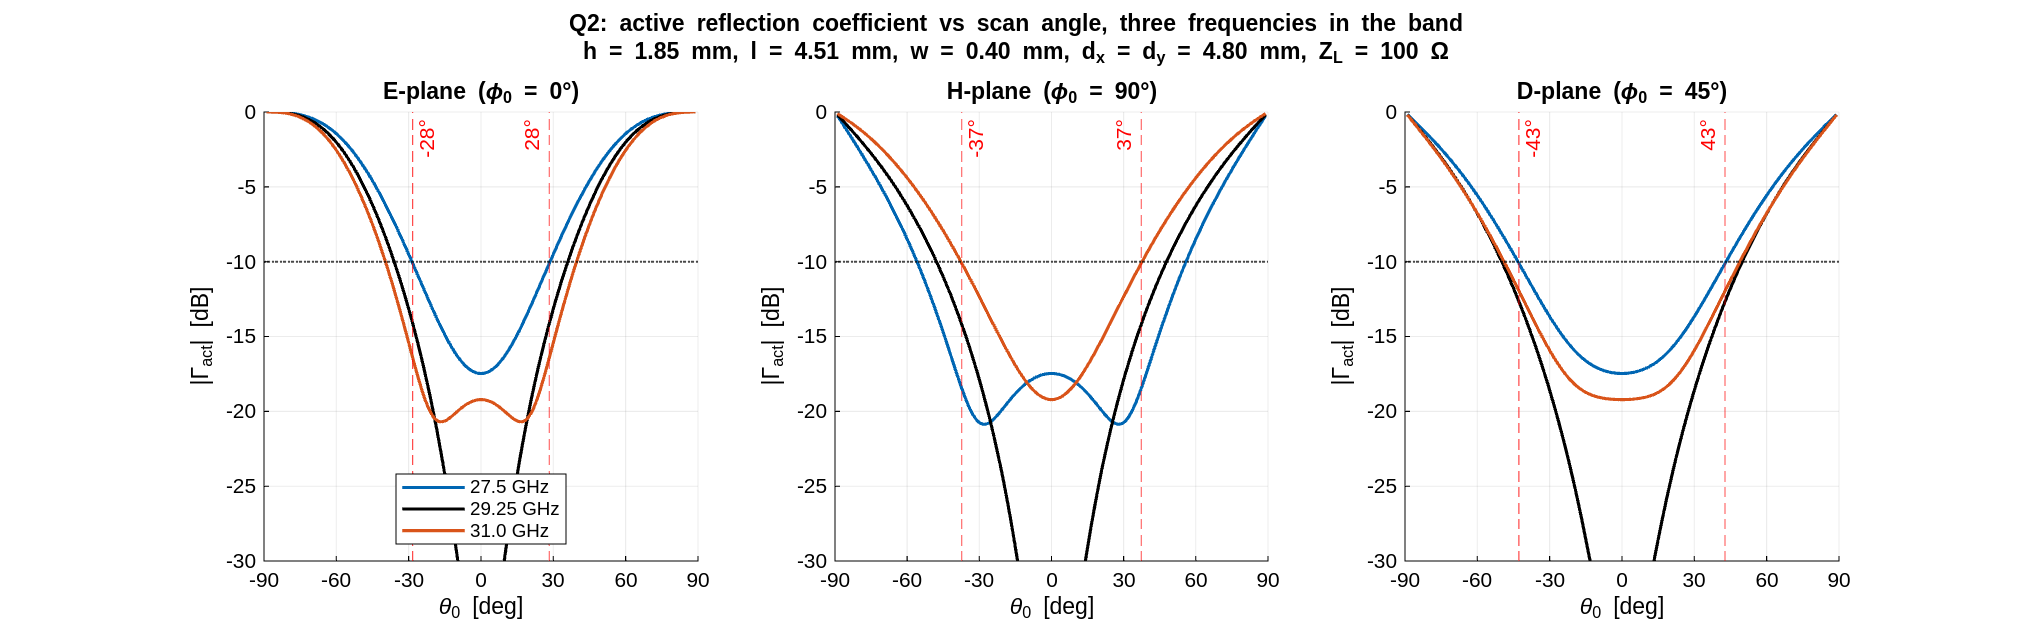
\includegraphics[width=0.95\textwidth]{Q2_Gamma_vs_scan.png}
\end{frame}
\note{Now to the actual scan question. I plotted the active reflection coefficient versus scan angle in all three principal planes — E, H, and D — at the two band edges and the centre. The three frequencies are colour-coded. The dashed red lines mark the scan angle where the worst case across all three frequencies crosses the minus-ten-decibel threshold. In the E-plane it is twenty-eight degrees, in the H-plane thirty-seven, and in the D-plane forty-three. The system-level scan limit is set by the worst plane and the worst frequency — that is twenty-eight degrees in the E-plane at thirty-one gigahertz. The curves are perfectly smooth — no Wood-anomaly spikes, exactly because the lattice is sub-half-wave at every frequency. The roll-off is just smooth scan loss.}

%================================================================
\begin{frame}{Q2 — Why is the E-plane the bottleneck?}
\textbf{Fundamental Floquet term} of $Z_{\text{in,act}}$ on the principal scan trajectory:
\[
Z_{00}(\theta_0) \;=\; \frac{\zeta_0}{2\,d_x d_y}\;\frac{k_0^2-k_{x0}^2}{k_0\,k_{z0}}\;\Bigl(1-e^{-j 2 k_{z0} h}\Bigr)\,[I(k_{x0})]^2
\]
\begin{columns}[T]
\column{0.5\textwidth}
\textbf{H-plane} ($k_{x0}=0$, $k_{y0}=k_0\sin\theta_0$)
\[ Z_{00} \propto \frac{1}{\cos\theta_0}\,(1-e^{-j 2k_0\cos\theta_0 h}) \]
$1/\cos\theta_0$ \emph{up}, reflector factor stays $\sim 2$ \\
$\Rightarrow$ Re$\{Z\}$ \emph{rises} smoothly, easy to keep matched.
\column{0.5\textwidth}
\textbf{E-plane} ($k_{x0}=k_0\sin\theta_0$, $k_{y0}=0$)
\[ Z_{00} \propto \cos\theta_0\,(1-e^{-j 2k_0\cos\theta_0 h})\,[I]^2 \]
$\cos\theta_0$ \emph{down} \emph{and} $I(k_{x0})$ rolls off with scan \\
$\Rightarrow$ Re$\{Z\}$ \emph{drops fast}, mismatch hits $-10\,$dB first.
\end{columns}
\vspace{6pt}
\centering
\textbf{Result:} system scan limit $\theta_{0,\max} \approx \pm 28^{\circ}$ across the full band (E-plane, $f_{hi}$).
\end{frame}
\note{It is worth understanding why the E-plane is the limiting plane, because students often expect the H-plane to be worse. Look at the closed form for the fundamental Floquet term. In the H-plane the scan moves along k y, k x stays zero, so the basis function transform is unchanged, and the only scan dependence is one over cos theta in the wave impedance — the resistance grows with scan angle. In the E-plane the scan moves along k x, which directly affects the basis Fourier transform, and the cos theta factor from the green function reduces the resistance instead of raising it. So in the E-plane the real part of Z drops below the matching window long before the reflector factor changes. That is why the E-plane scan limit is twenty-eight degrees — about ten less than the H-plane.}

%================================================================
\begin{frame}{Q3 — How many elements for HPBW $= 2^{\circ}$?}
\begin{columns}[T]
\column{0.42\textwidth}
\textbf{Closed form:}\\
uniform $N\times N$, broadside:
\[ \text{HPBW}\approx \frac{0.886\,\lambda}{N\,d}\;[\text{rad}] \]
For $\text{HPBW}=2^{\circ}$, $d=4.8$\,mm:
\renewcommand{\arraystretch}{1.05}
\begin{tabular}{cc}
\toprule
$f$ [GHz] & required $N$ \\
\midrule
27.5  & 58 \\
29.25 & \textbf{55} \\
31.0  & 52 \\
\bottomrule
\end{tabular}
\vspace{4pt}
\textbf{Recommendation:} $55\times 55 = 3025$ elements\\
(or $58\times 58$ for strict worst-case)
\column{0.58\textwidth}
\centering
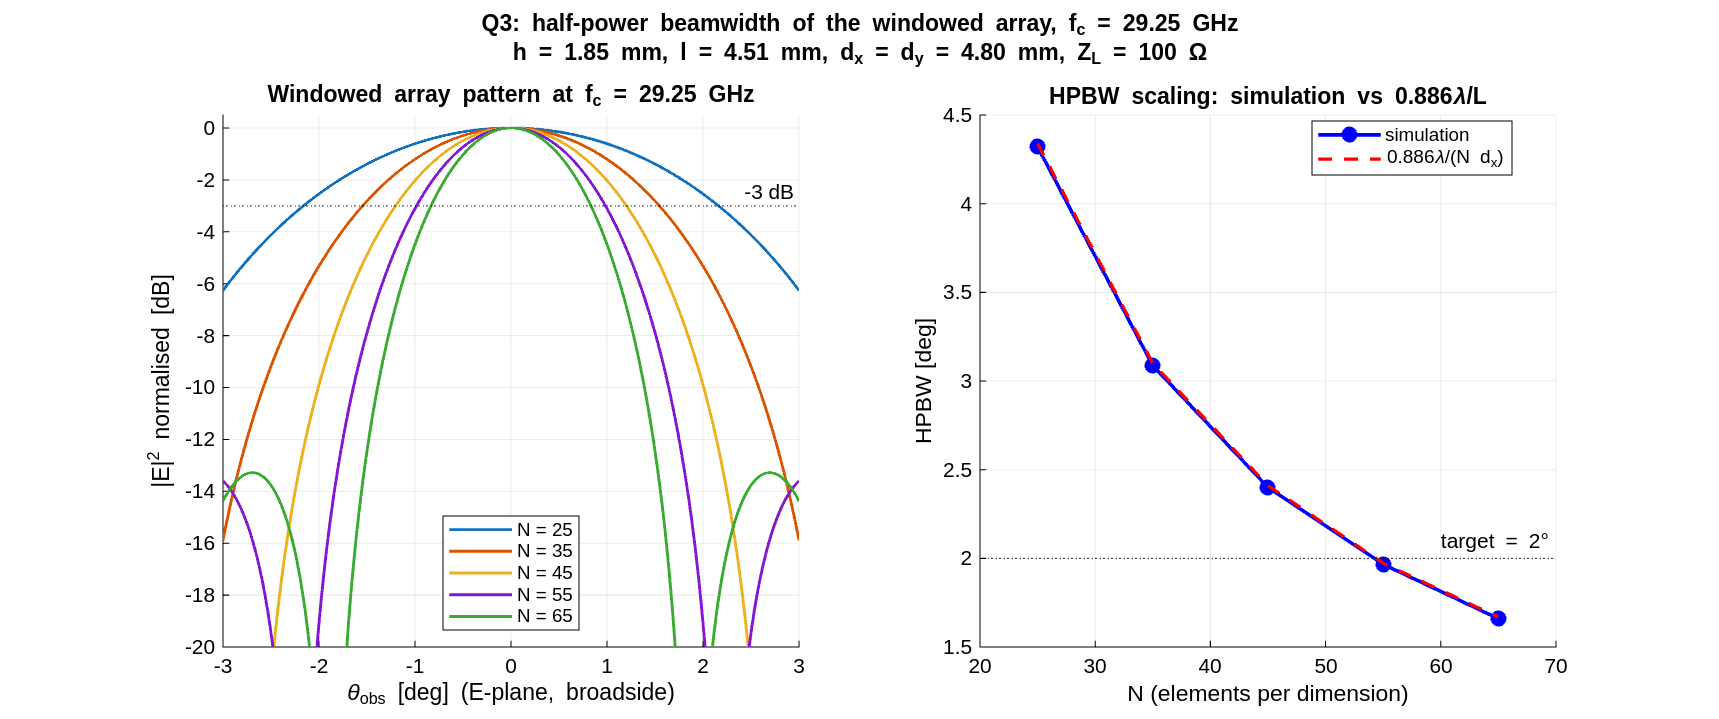
\includegraphics[width=0.99\textwidth]{Q3_HPBW.png}\\[2pt]
\small Simulation overlaps the closed-form $0.886\lambda/L$ exactly.
\end{columns}
\end{frame}
\note{Question three asks for the array size that delivers a two-degree half-power beamwidth. From the closed-form expression — zero point eight eight six lambda over array length — the worst case is the lowest frequency, where the wavelength is largest. The table shows fifty-eight elements at twenty-seven point five gigahertz, fifty-five at the centre, fifty-two at thirty-one. The figure is a numerical check. The left panel is the windowed array pattern at the centre frequency for several values of N; the right panel plots the simulated half-power beamwidth versus N alongside the closed-form curve. They overlap perfectly. Fifty-five elements per side gives one point nine six degrees at the centre frequency — just below the spec. So my recommendation is fifty-five by fifty-five, three thousand and twenty-five elements total. If you want strict worst-case compliance across the whole band you bump that to fifty-eight per side, which is three thousand three hundred and sixty-four elements.}

%================================================================
\begin{frame}{Q3 — Beamwidth across the band}
\begin{columns}[T]
\column{0.55\textwidth}
\centering
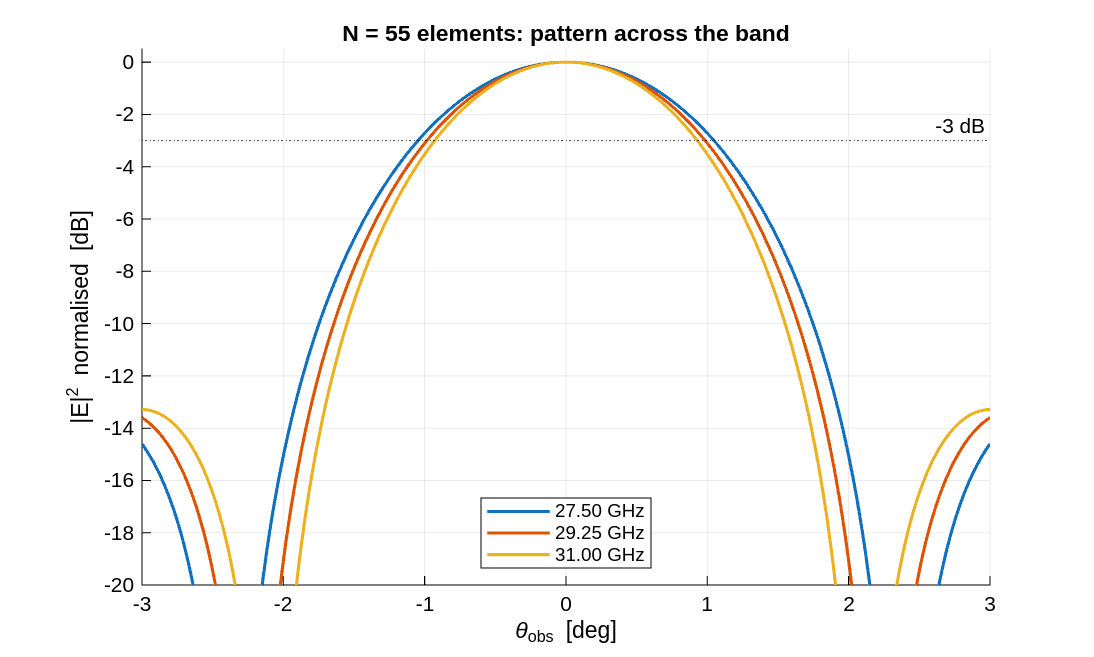
\includegraphics[width=0.99\textwidth]{Q3_HPBW_band.png}\\[2pt]
{\small Pattern of the chosen $55\times 55$ array.}
\column{0.45\textwidth}
\renewcommand{\arraystretch}{1.15}
\centering
\begin{tabular}{cc}
\toprule
$f$ [GHz] & HPBW [deg]\\ \midrule
27.5  & 2.09 \\
29.25 & 1.97 \\
31.0  & 1.85 \\ \bottomrule
\end{tabular}
\vspace{8pt}
\begin{itemize}
\item HPBW shrinks at higher $f$
\item $55{\times}55$ hits the spec at $f_c$, $4\%$ overshoot at $f_{lo}$
\item $58{\times}58$ guarantees the worst case
\end{itemize}
\end{columns}
\end{frame}
\note{One more chart for context. The half-power beamwidth varies inversely with frequency, so a fixed-size array gives different beamwidths across the band. The fifty-five-by-fifty-five design hits one point nine seven degrees at the centre, narrows to one point eight five degrees at thirty-one gigahertz, and widens to two point zero nine degrees at twenty-seven and a half. That is a four percent overshoot at the worst frequency — a non-issue from a system-engineering standpoint. If you really need every frequency under two degrees, the next square step is fifty-eight by fifty-eight, an extra three hundred and forty elements, or eleven percent more area.}

%================================================================
\begin{frame}{Conclusions}
\begin{enumerate}
\setlength\itemsep{4pt}
\item \textbf{Backing reflector via image theorem} ($\widetilde{G}_{xx,\text{eff}} = \widetilde{G}_{xx,\text{FS}}\bigl[1-e^{-j2k_z h}\bigr]$): the only mathematical change vs Assignments 5--6, drives the entire bandwidth and matching behaviour.
\item \textbf{Designed unit cell:} $h{=}1.85$\,mm, $l{=}4.51$\,mm, $w{=}0.4$\,mm, $d_x{=}d_y{=}4.8$\,mm, $Z_L{=}100\,\Omega$.\\
      Worst-case broadside $|\Gamma_{\text{act}}| = -17.5$\,dB ($7.5$\,dB below spec).
\item \textbf{Sub-half-wave lattice} guarantees no grating lobes and no scan blindness anywhere in the band.
\item \textbf{System scan limit:} $\theta_{0,\max} \approx \pm 28^{\circ}$ (E-plane at $f_{hi}$); H-plane $\pm 37^{\circ}$, D-plane $\pm 43^{\circ}$.
\item \textbf{Array sizing:} $55\times 55 = 3025$ elements deliver HPBW $=2^{\circ}$ at $f_c$. \textbf{58$\times$58 $=$ 3364 elements} for strict worst-case compliance.
\end{enumerate}
\vspace{4pt}
\centering
\textbf{Thank you --- questions?}
\end{frame}
\note{To wrap up. The whole project came down to one mathematical change — replacing the free-space Green's function by the image-theorem effective Green's function — and then sweeping the geometry within the constraints of a sub-half-wave lattice. The chosen unit cell hits minus seventeen and a half decibels at broadside, which leaves seven and a half decibels of margin. The array is grating-lobe-free and scan-blindness-free across the entire band. The scan limit is plus or minus twenty-eight degrees, set by the E-plane at the high band edge. And fifty-five by fifty-five elements deliver a two-degree pencil beam at the centre frequency, with fifty-eight by fifty-eight as the strict worst-case option. Thank you, I am happy to take questions.}

\end{document}
